% Created 2016-06-20 Mon 21:52
\documentclass[11pt]{article}
\usepackage[utf8]{inputenc}
\usepackage[T1]{fontenc}
\usepackage{fixltx2e}
\usepackage{graphicx}
\usepackage{grffile}
\usepackage{longtable}
\usepackage{wrapfig}
\usepackage{rotating}
\usepackage[normalem]{ulem}
\usepackage{amsmath}
\usepackage{textcomp}
\usepackage{amssymb}
\usepackage{capt-of}
\usepackage{natbib}
\usepackage[linktocpage,pdfstartview=FitH,colorlinks,
linkcolor=blue,anchorcolor=blue,
citecolor=blue,filecolor=blue,menucolor=blue,urlcolor=blue]{hyperref}
\usepackage{float}
\author{Steven Shaw}
\date{17-Jun-2016}
\title{Writing papers with Emacs, org-mode and org-ref}
\hypersetup{
 pdfauthor={Steven Shaw},
 pdftitle={Writing papers with Emacs, org-mode and org-ref},
 pdfkeywords={},
 pdfsubject={},
 pdfcreator={Emacs 24.4.51.2 (Org mode 8.3.4)}, 
 pdflang={English}}
\begin{document}

\maketitle

\section{Introduction}
\label{sec:orgheadline1}

Cite a paper \cite{hughes-why}.

Multiple citations \cite{not-a-number,why-dependent-types-matter}.

More citations \cite{ffi,secd,filinski-nbesem,nbe-filinski,rbtree}.

Alternative cites \citenum{hughes-why}.

\section{Methods}
\label{sec:orgheadline2}

\begin{equation} \label{eq-sinh}
y = \sinh x
\end{equation}

Refer to eq. \eqref{eq-sinh} for the details.

\section{Results}
\label{sec:orgheadline3}

\begin{figure}[H]
\centering
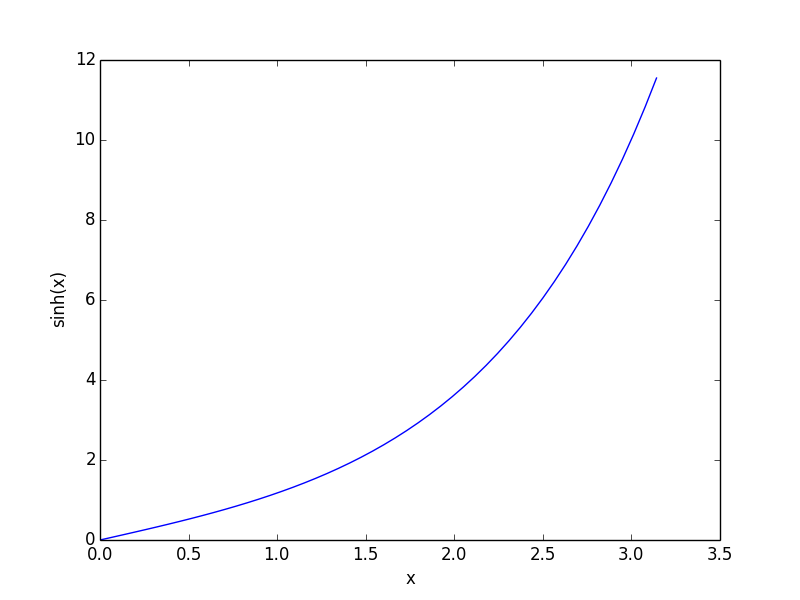
\includegraphics[width=.9\linewidth]{./sinh.png}
\caption{plotting is a cinch. \label{fig-cinch}}
\end{figure}

The results are in Figure \ref{fig-cinch}.

\section{Conclusions}
\label{sec:orgheadline4}

org-ref was used in these papers \cite{view-left,not-a-number,extt,mcbride-snr-thesis}.

It made it easy.

\bibliographystyle{unsrt}
\bibliography{manuscript,literature}
\end{document}